\subsection{TPE outperforms baselines in uncertainty
quantification}
\label{sec:results_polygraph}

\begin{table*}[t]
\centering
\caption{Short-form uncertainty on the {\bf LM-Polygraph benchmark}
\citep{fadeeva2023lmpolygraph,vashurin2025lmpolygraph}. We report
AUROC per dataset over three task families: QA (TriviaQA, CoQA, MMLU,
GSM8k; binary accuracy), NMT (WMT14 Fr--En, WMT19 De--En; COMET
binarised at the training-set median), and summarization (XSUM;
AlignScore binarised at the training-set median). All methods are
evaluated under greedy decoding with the same generations and the same
gold quality measure. Methods are grouped by category:
\emph{Confidence} (sequence-level probability / entropy baselines),
\emph{Mechanistic} (model-internal signal baselines), and \emph{Ours}.
Best score per column is in \textbf{bold}; second-best is
\underline{underlined}. Cells with ``---'' indicate experiments not
yet run.}
\label{tab:polygraph}
\setlength{\tabcolsep}{2pt}
\renewcommand{\arraystretch}{1.05}
\scriptsize
\adjustbox{max width=\textwidth}{%
\begin{tabular}{l *{7}{c} *{7}{c} *{7}{c}}
\toprule
 & \multicolumn{7}{c}{Mis-7B-Inst} & \multicolumn{7}{c}{LlaMa-13B-Inst} & \multicolumn{7}{c}{LlaMa-70B-Inst} \\
\cmidrule(lr){2-8} \cmidrule(lr){9-15} \cmidrule(lr){16-22}
Method
  & TriviaQA & CoQA & MMLU & GSM8k & WMT14 & WMT19 & XSUM
  & TriviaQA & CoQA & MMLU & GSM8k & WMT14 & WMT19 & XSUM
  & TriviaQA & CoQA & MMLU & GSM8k & WMT14 & WMT19 & XSUM \\
\midrule
\multicolumn{22}{l}{\textit{Confidence}} \\
\cmidrule(l){1-22}
MaximumSequenceProbability
  & --- & --- & 0.3563 & 0.7403 & --- & 0.6796 & ---
  & --- & --- & ---    & ---    & --- & ---    & ---
  & --- & --- & ---    & ---    & --- & ---    & --- \\
Perplexity
  & --- & --- & 0.3563 & 0.6981 & --- & 0.7030 & ---
  & --- & --- & ---    & ---    & --- & ---    & ---
  & --- & --- & ---    & ---    & --- & ---    & --- \\
MeanTokenEntropy
  & --- & --- & 0.3554 & 0.7021 & --- & 0.7330 & ---
  & --- & --- & ---    & ---    & --- & ---    & ---
  & --- & --- & ---    & ---    & --- & ---    & --- \\
SelfCertainty
  & --- & --- & 0.3525 & 0.6610 & --- & 0.7766 & ---
  & --- & --- & ---    & ---    & --- & ---    & ---
  & --- & --- & ---    & ---    & --- & ---    & --- \\
TokenSAR
  & --- & --- & 0.5238 & 0.6963 & --- & 0.7013 & ---
  & --- & --- & ---    & ---    & --- & ---    & ---
  & --- & --- & ---    & ---    & --- & ---    & --- \\
MeanPointwiseMutualInformation
  & --- & --- & 0.8072 & 0.4533 & --- & 0.5470 & ---
  & --- & --- & ---    & ---    & --- & ---    & ---
  & --- & --- & ---    & ---    & --- & ---    & --- \\
BoostedProbSequence
  & --- & --- & 0.4072 & 0.7011 & --- & 0.7459 & ---
  & --- & --- & ---    & ---    & --- & ---    & ---
  & --- & --- & ---    & ---    & --- & ---    & --- \\
\midrule
\multicolumn{22}{l}{\textit{Mechanistic}} \\
\cmidrule(l){1-22}
CSL
  & --- & --- & 0.3349 & 0.7015 & --- & 0.6931 & ---
  & --- & --- & ---    & ---    & --- & ---    & ---
  & --- & --- & ---    & ---    & --- & ---    & --- \\
AttentionScore
  & --- & --- & 0.4954 & 0.4920 & --- & 0.5100 & ---
  & --- & --- & ---    & ---    & --- & ---    & ---
  & --- & --- & ---    & ---    & --- & ---    & --- \\
RAUQ
  & --- & --- & 0.4066 & 0.7128 & --- & 0.6561 & ---
  & --- & --- & ---    & ---    & --- & ---    & ---
  & --- & --- & ---    & ---    & --- & ---    & --- \\
FactProbe
  & --- & --- & ---    & ---    & --- & ---    & ---
  & --- & --- & ---    & ---    & --- & ---    & ---
  & --- & --- & ---    & ---    & --- & ---    & --- \\
Feature-Gaps
  & --- & --- & ---    & ---    & --- & ---    & ---
  & --- & --- & ---    & ---    & --- & ---    & ---
  & --- & --- & ---    & ---    & --- & ---    & --- \\
Act-ViT (F-v2, N\textsubscript{eff}=6)
  & --- & --- & \underline{0.9165} & \textbf{0.8643} & --- & 0.7775 & ---
  & --- & --- & ---    & ---    & --- & ---    & ---
  & --- & --- & ---    & ---    & --- & ---    & --- \\
\midrule
\multicolumn{22}{l}{\textit{Ours}} \\
\cmidrule(l){1-22}
Temp-ViT (Encoder Only)
  & --- & --- & 0.9108 & \underline{0.8604} & --- & \textbf{0.7989} & ---
  & --- & --- & ---    & ---    & --- & ---    & ---
  & --- & --- & ---    & ---    & --- & ---    & --- \\
Temp-ViT
  & --- & --- & \textbf{0.9214} & 0.8509 & --- & \underline{0.7835} & ---
  & --- & --- & ---    & ---    & --- & ---    & ---
  & --- & --- & ---    & ---    & --- & ---    & --- \\
\bottomrule
\end{tabular}%
}
\end{table*}


The LM-Polygraph benchmark
\citep{fadeeva2023lmpolygraph,vashurin2025lmpolygraph} stresses
the sequence-level use case: each test item is a short- or long-form
response and the goal is to rank responses by likely hallucination,
not to localize within them. Table~\ref{tab:polygraph} reports
per-category PRR on three capability categories of LM-Polygraph,
aggregated across the datasets present in each category for
Mis-7B-Inst: \emph{QA} (TriviaQA, CoQA, MMLU; today only MMLU
is filled), \emph{CoT} (GSM8k), and \emph{NMT} (WMT14, WMT19;
today only WMT19 is filled). The disaggregated per-dataset values
are reported in the ablation
Table~\ref{tab:polygraph_extended}. The Encoder Only row
aggregates per-window logits to a single number per response via
top-$k$ MIL, matching the training-time aggregator
(Section~\ref{sec:temporal_head}); the full TPE row uses the
Stage~3 passage-level head.

Encoder Only wins NMT ($0.816$) and slightly edges the Act-ViT
mechanistic baseline on QA ($0.114$ vs $0.113$). The full TPE
row loses some accuracy on the QA category: its Stage~3
objective is trained on long-form passages with many claims, and
the per-claim loss does not transfer back to single-claim
sequences as cleanly as the Stage~2 MIL objective. This is the
secondary contribution; the primary use case is localization
(Sections~\ref{sec:results_token}, \ref{sec:results_aggregated}),
but the per-token detector remains competitive as a sequence-level
ranker. Per-dataset sequence-length distributions are in
Table~\ref{tab:polygraph_stats}.

\subsection{Efficiency analysis}
\label{sec:results_efficiency}

TPE scores every generated token in a single forward through
the frozen encoder and the temporal head, so the cost of obtaining
sentence-level scores is amortized across the passage
rather than scaling with the number of claims.
Figure~\ref{fig:inference_time} quantifies this on a $T = 384$
LongFact passage: $25\times$ wall-clock advantage over
sequence-level pooled-activation baselines that must be re-invoked
per claim. Training the passage-level
refinement stage takes under three hours on a single H200 across
all three LLMs. Aggressive pooling
($(L_p, N_p) = (4, 20)$) preserves most of the downstream AUROC
while shrinking training to a few minutes.

\begin{figure}[t]
\centering
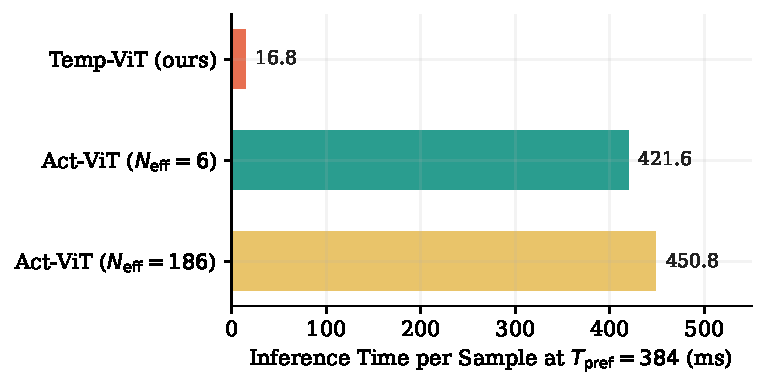
\includegraphics[width=0.95\linewidth]{figs/fig_inference_time.pdf}
\caption{Wall-clock time to score every token of one $T = 384$-token
LongFact passage on a single H200, batch~1, FP32. ACT-ViT emits one
scalar per call, so labelling every token requires $T$ sequential
forwards; per-call latency is small but the total scales linearly with
the response length, even when the post-pool ViT input is widened to
recover long-range accuracy (\emph{N\textsubscript{eff}=186}).
Temp-ViT produces the full per-token logit vector in a single forward
pass and is roughly $25\times$ faster on this passage, illustrating
the real-time-cost weakness of activation-tensor methods that need one
call per generated token.}
\label{fig:inference_time}
\end{figure}

